\section{Evaluation}
The specified CPA was implemented in CPAchecker\cite{Beyer2011} using the existing \compositeCPA\ and \locationCPA.
The existing \valueAnalysisCPA\ was extended to fulfil the specification of the \symbolicValueCPA,
while the constraints CPA was implemented as a new, individual CPA. To check the satisfiability of constraints, an external SAT solver is used.
For these benchmarks, MathSAT5 is used with the bitvector theory, encoding float values as floats.
The analysis is part of CPAchecker's trunk since revision 16052 and can be activated by using the configuration \texttt{valueAnalysis-symbolic}. Revision 16433 was chosen for benchmarks.

Benchmarks were performed on a subset of the SV-COMP 2015 test set, excluding sets CPAchecker's \valueAnalysisCPA\ has no support for.
These excluded sets are "Concurrency", "Memory Safety", "Recursive" and "Termination". An overview of all test sets can be found at \cite{SV15Tasks}.
Tests were executed on Intel Xeon E7-4870 machines at 2.40GHz with 80 cores and 322GB of available memory, with a memory limit of 15.0GB, a time limit of 900 seconds and a core limit of two CPUs per run.
A Java heap memory limit of 10.5GB per run was used.

All benchmark results are available at \url{http://leostrakosch.github.io/symbolicValueAnalysis}.

\begin{figure}[h]
\begin{tabular}{| r || r | r | r |}
\hline
                     & Value & SymEx & Overall \\ \hline
correct                & 1995 &  833 & 3038 \\ \hline
true positives         &  632 &  246 &  802 \\ \hline
true negatives         & 1363 &  587 & 2236 \\ \hline
unique true positives  &  393 &    7 &    - \\ \hline
unique true negatives  &  804 &   28 &    - \\ \hline
false positives        &  271 &   52 &    - \\ \hline
unique false positives &  222 &    3 &    - \\ \hline
false negatives        &    0 &    0 &    - \\ \hline 
timeouts               &  662 & 1970 &    - \\ \hline
errors                 &  110 &  182 &    - \\ \hline
memory errors          &    0 &    1 &    - \\ \hline
\end{tabular}
\caption{Result of runs of value analysis (Value) and symbolic execution (SymEx) on SV-COMP 2015 test sets.
  "true positive" represents a found property violation in a program containing a property violation,
  "true negative" represents no found violation in a program without violations.}
\label{tab:diff}
\end{figure}
Figure \ref{tab:diff} shows the performance of the default \valueAnalysisCPA\ without counterexample-guided abstraction refinement (CEGAR \cite{Beyer2013}) or counterexample checks next to the performance of the new symbolic execution configuration.
Generally speaking, basic value analysis strongly outperforms symbolic execution in numbers due to symbolic execution taking too long.
Lots of timeouts occur due to
(a) path explosion, an exponential increase in possible paths based on the number of branches (that is if-statements and loops) as a result of the low level of abstraction of symbolic execution, and
(b) the bad performance of SAT checks with a large number of variables and arithmetic operations like non-linear multiplication.
Path explosion can easily be illustrated when looking at the algorithm statistics of a simple program using multiple if- and goto-statements.\footnote{Namely program \texttt{ldv-validator-v0.6/linux-stable-9ec4f65-1-110\_1a-drivers--rtc--rtc-tegra.ko-entry\_point\_false-unreach-call.cil.out.c}}
While basic value analysis only needs 1241 iterations to find a possible property violation, with the biggest waitlist consisting of 42 entries,
analysis with symbolic execution needs 14572 iterations with the biggest waitlist consisting of 543 states to find the same property violation.
The scatter plot in Figure \ref{graph:computedSuccessors} displays this problem.
For some tasks, symbolic execution is able to compute the result with less successors than value analysis due to its stronger precision. But in many cases, symbolic execution computes far more successors because of this.
\begin{figure}[h]
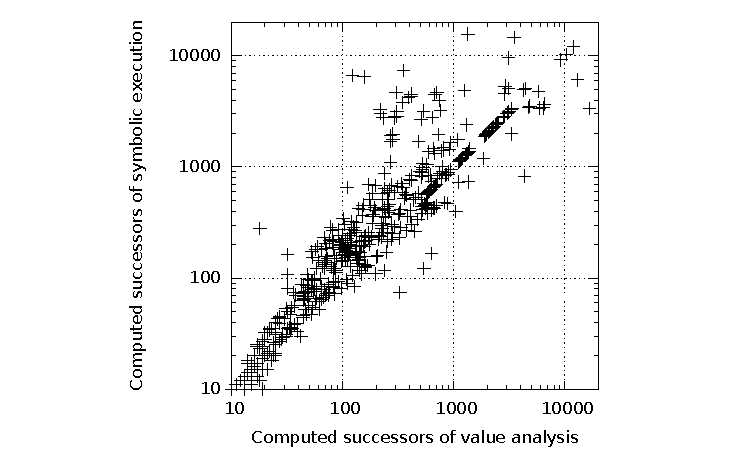
\includegraphics[width=\linewidth]{sp_reachedSetsOnTerminatedAndEqualResults_symbolic_explicit}
\caption{Number of computed successors for \valueAnalysisCPA\ and \symbolicExecutionCPA.
         Only the computed successors for benchmark runs are displayed which returned a result for both \symbolicExecutionCPA\ and \valueAnalysisCPA\ and for which the result was the same. The upper bound used for computed successors is 20,000.}
\label{graph:computedSuccessors}
\end{figure}
In addition to this enormous growth in iterations, SAT checks are responsible for up to 95.0\% of CPU time in analyses of programs using non-deterministic values that are \emph{not} specifically constructed for challenging SAT solvers.
This influences the speed at which successors can be computed.
As can be seen in Figure \ref{graph:computedSuccessorsPerS}, there are many benchmark runs in which \valueAnalysisCPA\ is able to compute significantly more successors per second (in average) than \symbolicExecutionCPA.
\begin{figure}[h]
\includegraphics[width=\linewidth]{sp_computedSuccessorsPerSecond_symbolic_explicit}
\caption{Number of computed successors per second for \valueAnalysisCPA\ and \symbolicExecutionCPA}
\label{graph:computedSuccessorsPerS}
\end{figure}

Despite this reduced speed, symbolic execution's ability to track non-deterministic values allows it to get a correct result in 35 cases in which value analysis does not. In seven of these value analysis exceeds the timelimit and in 28 value analysis provides a false positive. Symbolic execution does never produce a false result when value analysis produces a correct one.

When using a timelimit of 1800 seconds, symbolic execution is able to compute 9 more results than with a timelimit of 900 seconds, of which seven are correct.

Of these long-taking runs, three are the result of path explosion,
while the other five only consist of few iterations, but contain expressions resulting in long-taking SAT checks, namely bitvector computations, non-deterministic floats and non-linear multiplications.

These performance issues can be improved by using another theory in SAT checks.
By using an integer theory instead of bitvector, runtime can be greatly improved in some cases.
The scatter plot in Figure \ref{graph:bitvecIntCompGraph} illustrates the runtime improvements of integer theory over bitvector.
This results in a lower precision and an unsound analysis, though.
Figure \ref{tab:bitvecIntComp} shows the difference between the use of a bitvector theory with floats and the use of an integer theory.
\begin{figure}[h]
\begin{tabular}{| r || r | r |}
\hline
& Bitvector theory & Integer theory \\ \hline
correct         &  833 &  815 \\ \hline
false positives &   52 &   93 \\ \hline
false negatives &    0 &    5 \\ \hline
timeouts        & 1970 & 1944 \\ \hline
errors          &  182 &  175 \\ \hline
memory errors   &    1 &    1 \\ \hline
\end{tabular}
\caption{Results of \symbolicExecutionCPA\ using bitvector theory with floats and integer theory on SV-COMP 2015 test sets.}
\label{tab:bitvecIntComp}
\end{figure}

\begin{figure}[h]
\includegraphics[width=\linewidth]{sp_performanceOnEqualAndTerminatedResults_integer_bitvector_theory}
\caption{Runtime performance of symbolic execution using an integer theory in comparison to bitvector + float theory.
\label{graph:bitvecIntCompGraph}
         Only benchmark runs that returned a result and for which the result of integer and bitvector was the same are
         displayed.}
\end{figure}

\section{Conclusion}
By extending the existing \valueAnalysisCPA\ with the ability to track non-deterministic values and the introduction of the new \constraintsCPA,
we were able to reduce the number of false positives of value analysis without the need for counterexample checks.
In contrast to predicate analysis, we take advantage of the value analysis's high performance with explicit values and only create boolean formulas when non-deterministic values occur.
As a downside, symbolic execution, as it is based on value analysis, is far less potent in handling pointers than predicate analysis.
But since this is only a very basic implementation, the potential of symbolic execution in the context of configurable software verification has still to be explored.

When choosing a SMT theory,
the trade-off between performance and precision
must be considered depending on the program's use of floats and bitwise operations.
To decrease runtime without a loss of precision, the problem of path explosion should be tackled.
A valid approach to this could be CEGAR, which is already implemented for the \valueAnalysisCPA.
The introduction of compact symbolic execution as described in \cite{Slaby2013} could be another useful extension to allow more efficient handling of loops.
By resolving the problem of path explosion, the number of iterations and as such also the number of SAT checks could be decreased, while keeping the high level of precision of symbolic execution.
A preliminary implementation of CEGAR with symbolic execution already shows high potential.
Refining this approach will be the main focus of future work.
